




\chapter{Práctica 3: Medidas en Corriente Alterna}

\section{Objetivos}
En esta práctica, se va a aprender a manejar el osciloscopio, y se estudiará un circuito RC. En él, se va a medir la diferencia de potencial en los extremos del condensador en función de la frecuencia de la señal de entrada. Posteriormente, se va a representar la función de transferencia del circuito RC tomando la salida en el condensador.

\section{Fundamento Teórico}
El circuito a tratar en esta sesión es un circuito RC (Figura \ref{fig:CircuitoRC}). En él, se encuentra una resistencia en serie con un condensador.

\begin{figure} [H]
    \centering
    \begin{circuitikz}
        \draw (0,0)
        to [ american resistor,  l=$R$ ] (3, 0)
        to [ capacitor] (3,-2)
        to [ short ] (0,-2)
        to[ vsourcesin, l=$v_i(t)$ ] (0,0);

        \draw
        (0, -0.3) node [left] {$+$}
        (0, -1.7) node [left] {$-$}
        (2.5, -1) node [left] {$C$};

        \draw (3.5,0) node [right] {$+$}
        (3.5,-2) node [right] {$-$}
        (3.5,-1) node [right] {$v_o(t)$};
        
    \end{circuitikz}
    \caption{Circuito RC}
    \label{fig:CircuitoRC}
\end{figure}


La función de transferencia $T(\omega)$ del circuito toma como entrada el potencial de entrada $V_i$ y como potencial de salida la caída de potencial en el condensador, $V_o$.
\begin{equation}
    T(\omega) = \frac{v_o(\omega)}{v_i(\omega)}
\end{equation}

Como la resistencia y el condensador del circuito están en serie,
\begin{equation}
    Z_{eq}=Z_R + Z_C = R + \frac{1}{j\omega C} = \frac{1+j\omega RC}{j \omega C}
\end{equation}

Por tanto, la intensidad de la corriente que circula por el circuito en sentido horario es:
\begin{equation}
    i(\omega) = \frac{v_i(\omega)}{Z_{eq}}=v_i(\omega) \frac{j \omega C}{1+j\omega RC}
\end{equation}

De esta forma, el potencial de salida $v_o(\omega)$ buscado es:
\begin{equation}
    v_C (\omega) = i(\omega)Z_C = v_i(\omega) \frac{\cancel{j \omega C}}{1+j\omega RC}\frac{1}{\cancel{j\omega C}}=v_i(\omega) \frac{1}{1+j\omega RC}
\end{equation}

Por tanto, la función de transferencia de este circuito queda:
\begin{equation} \label{Eq:FuncTrans}
    T(\omega) =  \frac{v_C(\omega)}{v_i(\omega)} = \frac{1}{1+j\omega RC}
\end{equation}

Como en esta práctica se va a representar el diagrama de Bode en módulo de la función de transferencia, se convierte la expresión compleja de $T(\omega)$ a polar:
\begin{equation}
    T(\omega) = \frac{1e^{j0}}{\sqrt{1 + (\omega RC)^2}e^{j\arctan(\omega RC)}} = \frac{1}{\sqrt{1 + (\omega RC)^2}} e^{-j\arctan(\omega RC)}
\end{equation}

Por tanto, la expresión a representar en el eje vertical del diagrama de Bode en módulo es:
\begin{equation}
    |T(\omega)|_{dB} = 20\log(|T(\omega)|) = 20\log\left( \frac{1}{\sqrt{1 + (\omega RC)^2}} \right)
\end{equation}

Para obtener la frecuencia de corte teórica del circuito, comparamos la función de transferencias obtenida (Ec. \ref{Eq:FuncTrans}) con la función de transferencia conocida $T(\omega) = \frac{1}{1+j\frac{\omega}{\omega_0}}$, donde obtenemos que:
\begin{equation}\label{Ec:FrqTeo}
    \omega_0 = \frac{1}{RC}
\end{equation}

Para obtener la frecuencia de corte experimental, hemos de establecer la condición de $\omega = \omega_0$. Por tanto, como indica la Ec. \ref{Ec:FrqExp}, hemos de buscar un valor donde el cociente entre la señal de salida entre la de entrada sea de aproximadamente $0.7$.
\begin{equation}\label{Ec:FrqExp}
    \omega = \omega_0 \Longrightarrow |T(\omega)|=\frac{1}{\sqrt{1+\frac{w_0}{w_0}}} = \frac{1}{\sqrt{2}}\approx 0.7
\end{equation}

En la figura \ref{Img:FuncTrans} se puede ver el diagrama de Bode en Módulo de la función de transferencia de este circuito (Ec. \ref{Eq:FuncTrans}). Como podemos ver, sus propiedades son:
\begin{itemize}
    \item \textbf{Si} $\mathbf{\omega \ll \omega_0}$ \textbf{:} No se modifica prácticamente la señal de entrada. La pendiente de esta zona es $0$.
    \item \textbf{Si} $\mathbf{\omega \approx \omega_0}$ \textbf{:} La atenuación es de -3 dB.
    \item \textbf{Si} $\mathbf{\omega \gg \omega_0}$ \textbf{:} La atenuación es cada vez mayor, ya que conforme aumenta la frecuencia disminuye la amplitud del potencial de salida. La pendiente de esta zona es $-1$.
\end{itemize}
Por tanto, como las frecuencias bajas no las modifica, este circuito se llama también \textbf{filtro paso baja}.

\begin{figure}
    \centering
    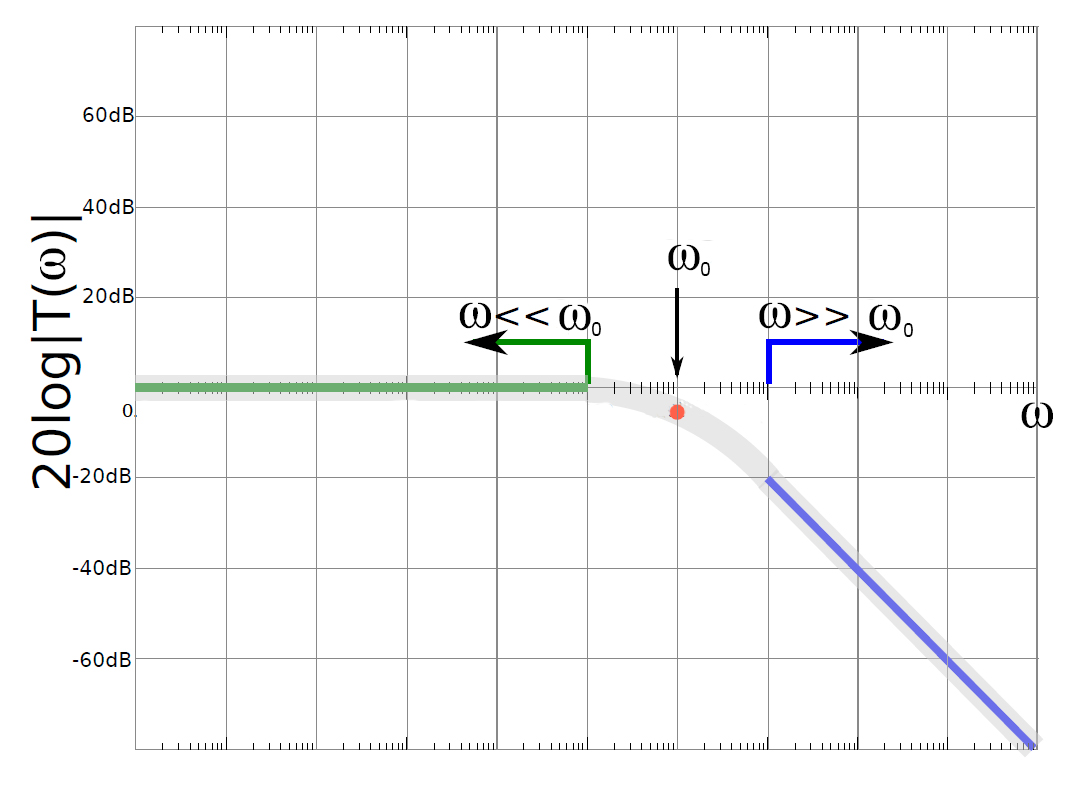
\includegraphics[width=10cm]{Imágenes 03/Funcion_De_Transferencia.jpg}
    \caption{Diagrama de bode en módulo de $T(\omega)$}
    \label{Img:FuncTrans}
\end{figure}

\section{Material}
\begin{itemize}
    \item \underline{Generador de Señales:} fuente de tensión de corriente alterna empleada para proporcionarle tensión al circuito RC. El modelo empleado es Agilent 33220A.
    \item \underline{Osciloscopio:} dispositivo empleado para realizar diversas medidas en el circuito. Permite ver las señales sinusoidales en pantalla. El modelo empleado es Agilent 54622A.
    \item \underline{Resistencia}
    \item \underline{Condensador}
    \item \underline{Protoboard}
\end{itemize}


\section{Desarrollo y resultados}
Los valores de los elementos empleados en el circuito son:
\begin{itemize}
    \item $R = 9.04\;k\Omega$
    \item $C = 1.985\;nF$
\end{itemize}
Una vez medidos estos, se han medido diversas magnitudes conforme se variaba la frecuencia de la señal de entrada. Los datos obtenidos se muestran en la figura \ref{fig:03.Datos}, donde cada columna representa:
\begin{description}
    \item [Columna 1:] Frecuencia teórica de la señal de entrada [$Hz$]. Dada por el generador de señales.
    \item [Columna 2:] Frecuencia experimental de la señal de entrada [$Hz$]. Medida por el osciloscopio.
    \item [Columna 3:] Frecuencia angular de la señal de entrada [$\frac{rad}{s}$]. $\omega = 2\pi f$
    \item [Columna 4:] Potencial de entrada pico a pico ($V_{ipp}$) [$V$]. Medido por el osciloscopio.
    \item [Columna 5:] Potencial de salida pico a pico ($V_{opp}$) [$V$]. Medido por el osciloscopio en los extremos del condensador.
    \item [Columna 6:] Módulo de la función de transferencia $\left(|T(\omega)| = \frac{|V_{opp}|}{|V_{ipp}|}\right)$.
    \item [Columna 7:] $20\log(|T(\omega)|)$ [dB]. Valores del eje vertical en el diagrama de Bode en módulo de la función de transferencia.
\end{description}

\begin{figure}
    \centering
    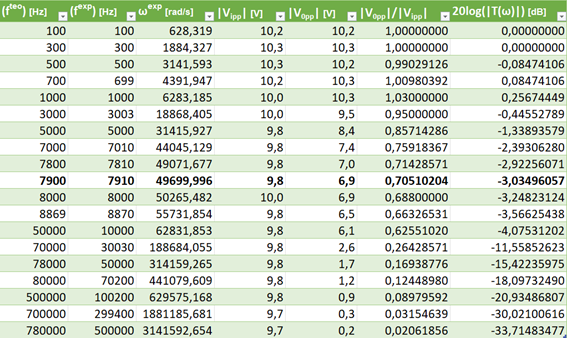
\includegraphics[width=13.5cm]{Imágenes 03/Tabla_Datos_Exp.png}
    \caption{Datos obtenidos con el circuito RC}
    \label{fig:03.Datos}
\end{figure}


En la figura \ref{fig:BodeExp} podemos ver el diagrama de Bode en módulo.
\begin{figure}
    \centering
    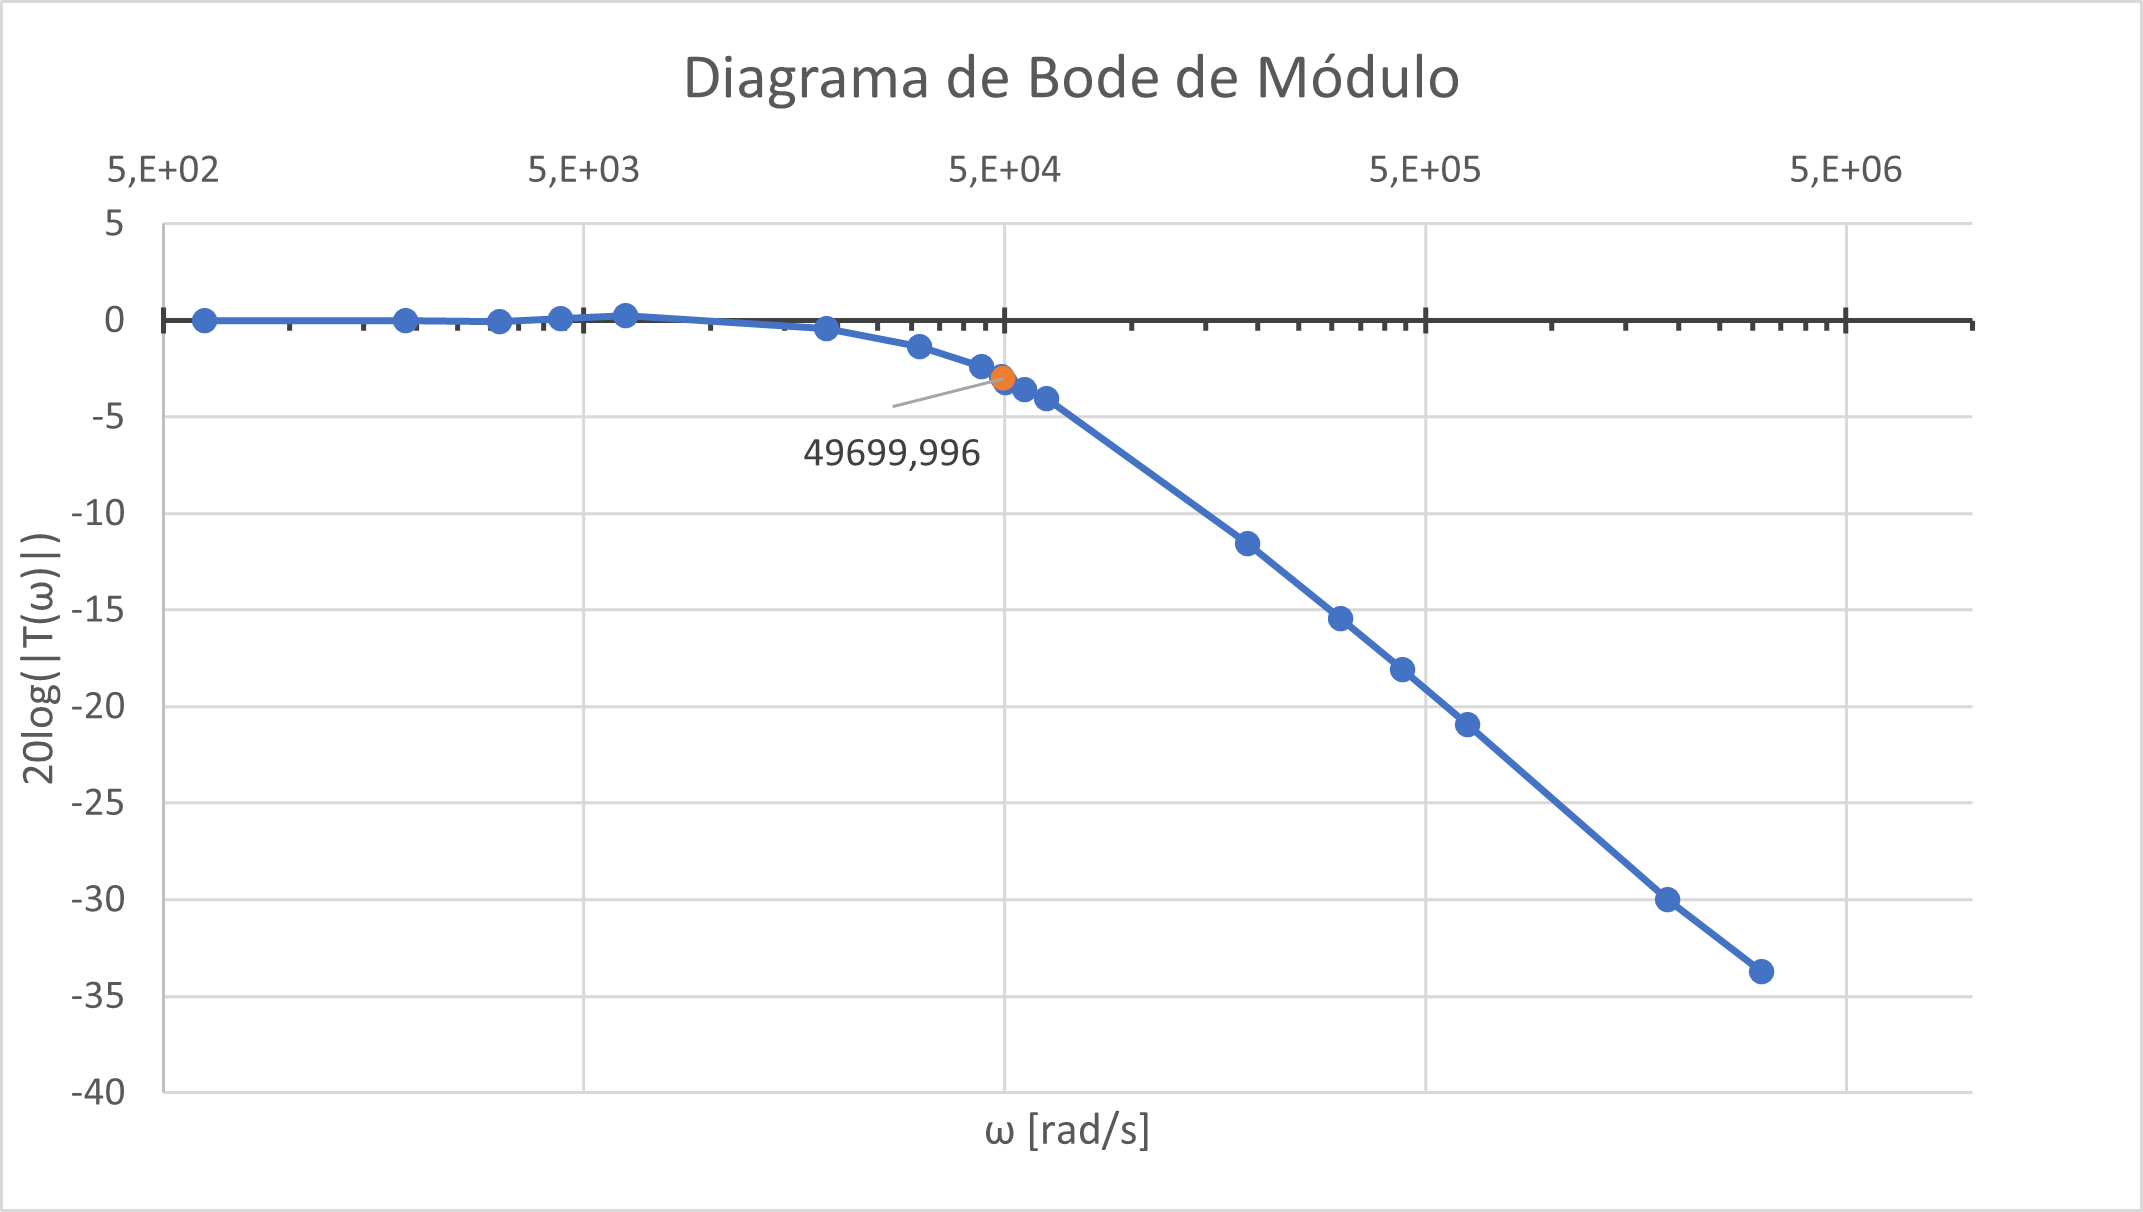
\includegraphics[width=13.5cm]{Imágenes 03/Grafico_Exp.png}
    \caption{Diagrama de Bode en módulo experimental}
    \label{fig:BodeExp}
\end{figure}

\section{Discusión}

\subsection{Frecuencia angular de corte}

En primer lugar, estudiamos \textbf{la frecuencia angular de corte}, tanto teórica como experimentalmente.

Según dice la teoría, como se ha visto en la Ec. \ref{Ec:FrqTeo}, la frecuencia de corte teórica es:
\begin{equation}
    \omega_o^{teo} = \frac{1}{RC} = 55727.69 \;\frac{rad}{s}
\end{equation}

En la práctica, según la Ec. \ref{Ec:FrqExp}, 
\begin{equation}
    \omega_0^{exp} = \omega / |T(\omega)| \approx 0.7 \Longrightarrow \omega_0^{exp} = 49699.996\;\frac{rad}{s}.
\end{equation}

Por tanto, como podemos ver, son resultados muy similares. La frecuencia de corte experimental es menor, lo que podría deberse a pérdidas de energía en las conexiones de la protoboard, imprecisiones en las mediciones, e incluso a que no se ha obtenido el valor exacto de $1\sqrt(2)$, sino que se ha aproximado a $0.7$.

\subsection{Gráfica de la función de transferencia}
Respecto a la gráfica de la \textbf{función de transferencia}, en la figura \ref{fig:Datos_Teo} se pueden ver los datos teóricos del módulo de la función de transferencia, y en la figura \ref{fig:BodeTeo} se puede ver una comparación del diagrama de Bode en módulo teórico y experimental. Es fácil ver la teoría se ajusta mucho a lo que sucede en la realidad, ya que ambas gráficas se solapan casi en su totalidad. Además, podemos ver que la frecuencia de corte teórica y experimental, aunque distintas, en el orden de magnitud en cuestion el error es prácticamente insignificante, ya que en la distancia que les separa en la gráfica es despreciable. Por último, vemos que los puntos en los que difieren se encuentran en las frecuencias más altas, y esto se debe a las imprecisiones del osciloscopio al requerir el uso del botón de \emph{trigger}.

\begin{figure}
    \centering
    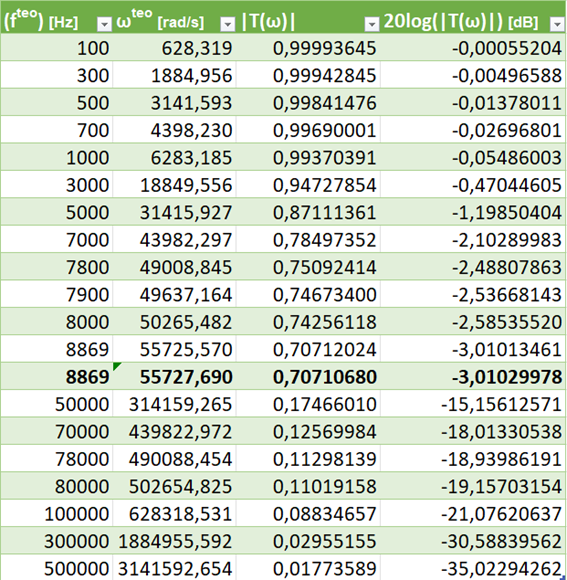
\includegraphics[width=8.5cm]{Imágenes 03/Tabla_Datos_Teo.png}
    \caption{Datos teóricos de este circuito RC}
    \label{fig:Datos_Teo}
\end{figure}

\begin{figure}
    \centering
    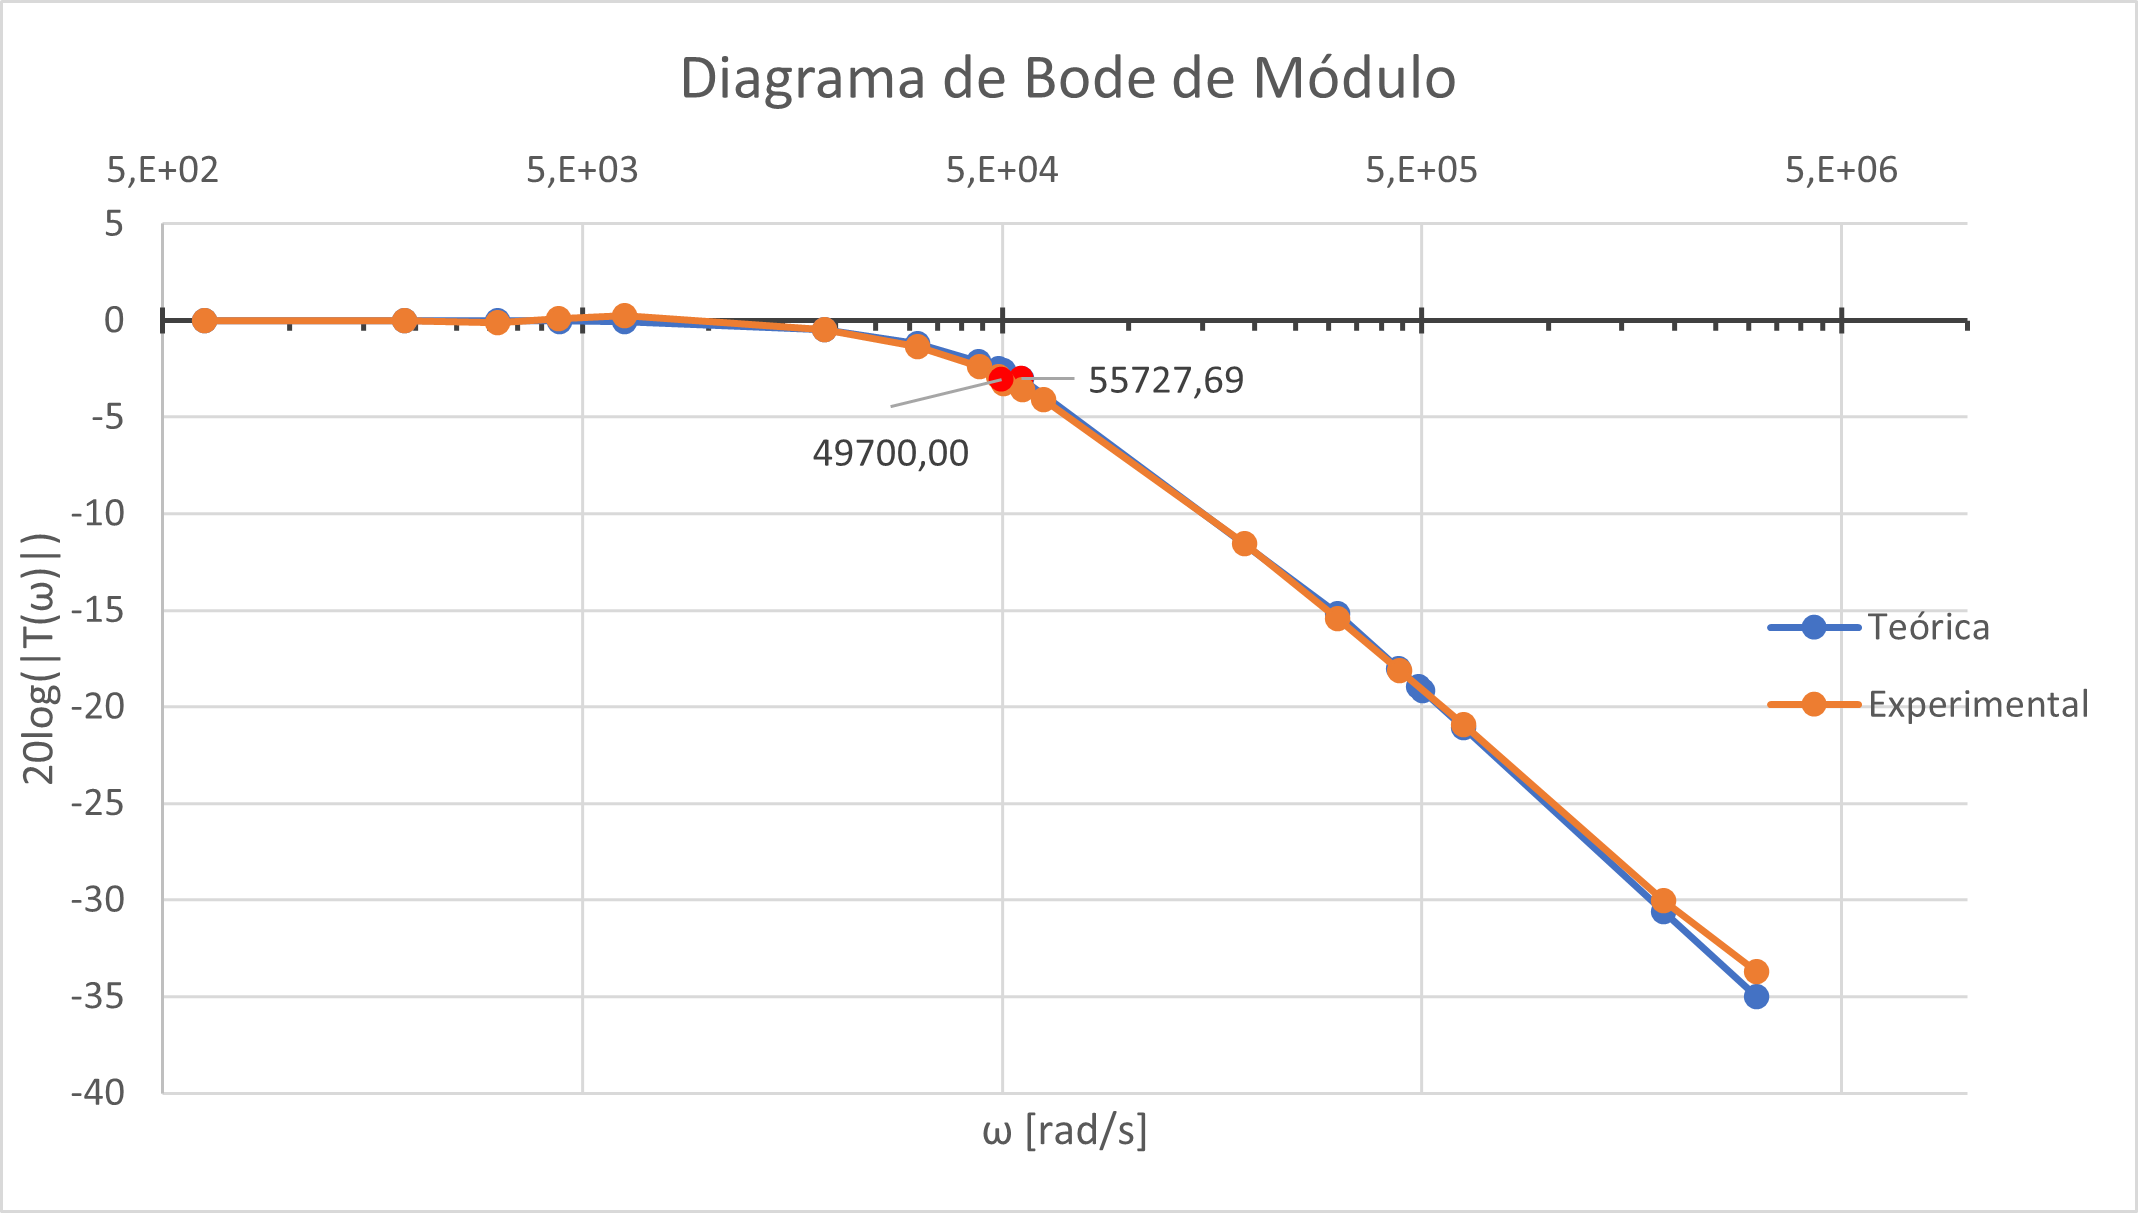
\includegraphics[width=13.5cm]{Imágenes 03/Grafico_Teo.png}
    \caption{Diagrama de Bode en módulo teórico y experimental}
    \label{fig:BodeTeo}
\end{figure}


\subsection{Pendiente de la zona con frecuencias altas}
Por último, vamos a calcular la pendiente de la zona descendiente del diagrama de Bode, aquella que se da para frecuencias mucho mayores que la de corte. En la figura \ref{fig:LinTen}, se puede observar que la linea de tenencia logarítmica de la parte en cuestión es $y=-7.44\ln{x} + 77.525$. Su coeficiente de correlación, $R^2 = 0.9973$, es cercano a 1, por lo que el ajuste es considerablemente correcto.

\begin{figure}
    \centering
    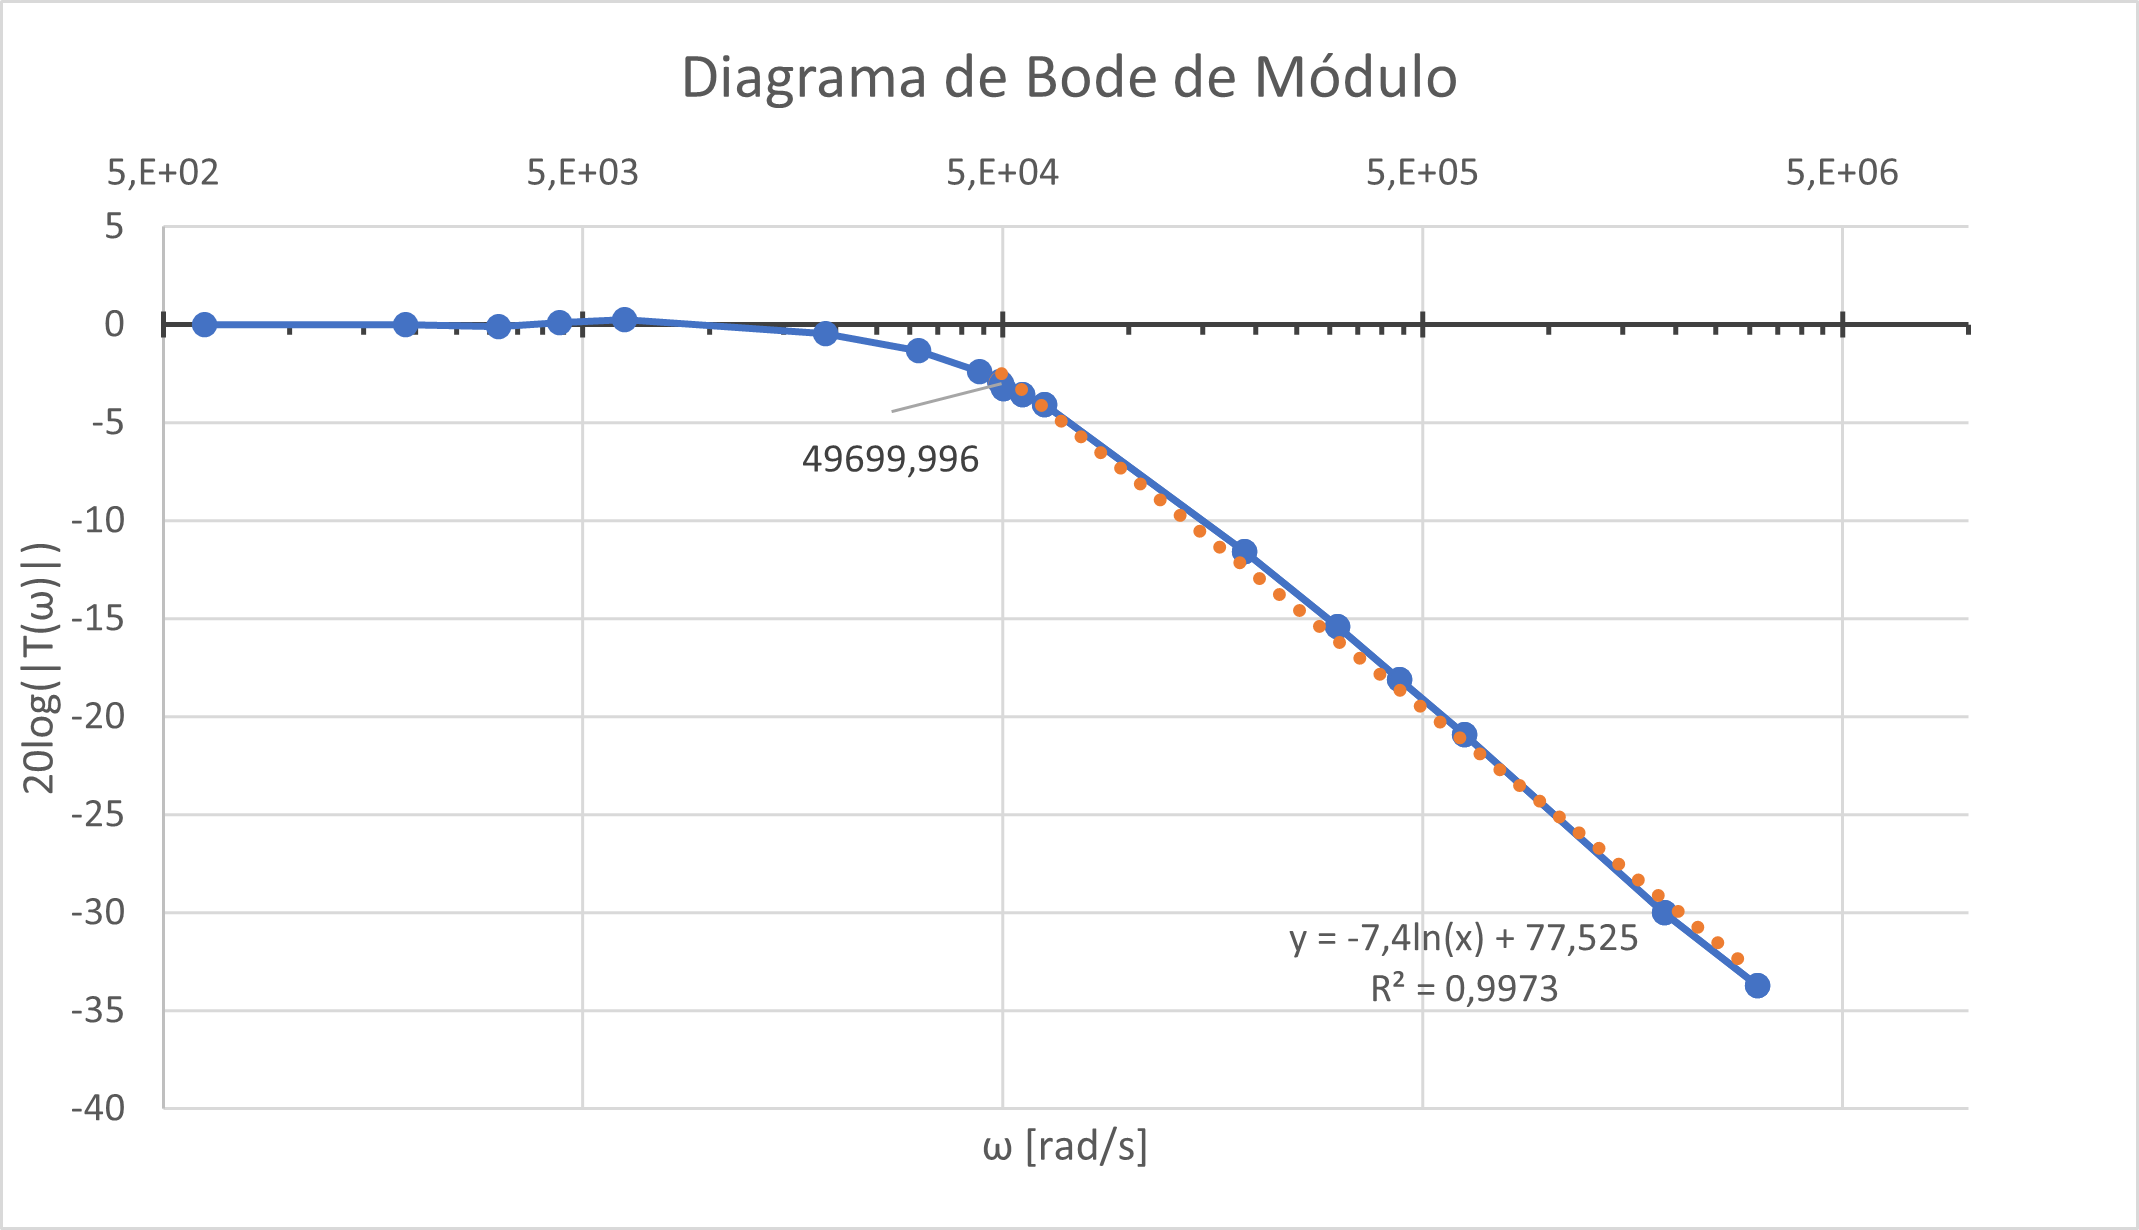
\includegraphics[width=13.5cm]{Imágenes 03/Linea_Tendencia.png}
    \caption{Línea de tendencia de las frecuencias altas del D. Bode}
    \label{fig:LinTen}
\end{figure}

Como se desea obtener una recta del tipo $y=m(20\log x)+n$, usamos el cambio de base para expresar el logaritmo de la linea de tendencia en base decimal.
\begin{equation}
\begin{split}
    y & = -7.44 \ln{x} + 77.525 = -7.44 \; \frac{\log(x)}{\log(e)} + 77.525 = \\
      & = -17.13 \log x + 77.525   \\
      & = -0.85 \; (20 \log x)+77.525
\end{split}
\end{equation}

Por tanto, la pendiente es $m^{exp}=-0.85$, que difiere de la teórica, que es $m^{teo} = -1$. Esto se puede deber a los puntos últimos de la recta, que como hemos mencionado antes difieren en mayor medida de la teoría.


\section{Conclusiones}
Las conclusiones extraídas de esta práctica de laboratorio son:
\begin{itemize}
    \item En primer lugar, se aprecia perfectamente que la teoría se ajusta en gran medida a lo que sucede experimentalmente, ya que los resultados que hemos obtenido ya habían sido predichos por la teoría anteriormente. Esto nos permite estudiar este tipo de circuitos teóricamente, sin tener que medir en ellos siempre. Cabe notar que los métodos teóricos utilizados son simplificaciones ideales de lo real, ya que en las medidas interfieren otros factores como el ruido o los errores de precisión humanos.
    
    \item En base a los resultados obtenidos, también se puede deducir que, en valores más límite como frecuencias muy altas, la teoría y lo experimental difieren más, y esto puede tener muchos motivos diversos. El más factible podría ser errores de precisión en los dispositivos empleados, como el error en el osciloscopio previamente mencionado.

    \item Por último, se ha podido comprobar que el circuito RC tomando como salida el condensador es, efectivamente, un filtro paso bajo, ya que solo deja pasar las frecuencias bajas y, sin embargo, atenúa en gran medida las frecuencias altas. Esto tendrá diversas aplicaciones e la ingeniería, como los ecualizadores de sonido.
\end{itemize}
